\section{Polygram Cipher}
\label{sec:polygram}

Polygram cipher melakukan substitusi pada \emph{blok huruf} (bukan huruf
tunggal). Karena yang dipetakan adalah rangkaian dua atau tiga huruf sekaligus,
sebaran frekuensi bigram dan trigram pun ikut tersembunyi: huruf \code{E} pada
posisi ganjil dan genap dapat berubah menjadi huruf yang berbeda, sehingga
puncak frekuensi huruf tunggal maupun pasangannya tidak lagi tampak jelas.
Dua wakil terpenting pendekatan ini adalah Playfair cipher, yang bekerja pada
bigram, dan Hill cipher, yang bekerja pada blok $m$ huruf melalui operasi
aljabar linier.

\subsection{Playfair Cipher}
\label{sec:playfair}

Playfair cipher bekerja pada unit \textbf{bigram}, yaitu pasangan dua huruf.
Cipher ini dirancang oleh Sir Charles Wheatstone sekitar 1854, tetapi
dipopulerkan oleh Baron Lyon Playfair --- seorang ilmuwan dan politikus yang
membantu menyebarkannya kepada kalangan militer Inggris --- sehingga namanya
yang dilekatkan pada cipher tersebut. Cipher ini dipakai oleh pasukan Inggris
pada Perang Boer dan Perang Dunia I karena dapat dihitung dengan cepat tanpa
alat bantu \citep{stinson2018}.

\textbf{Matriks kunci.} Kunci Playfair disusun dalam matriks $5 \times 5$.
Karena matriks itu hanya memuat 25 sel, sedangkan alfabet Latin berjumlah 26
huruf, satu huruf harus dikorbankan. Huruf yang dikorbankan adalah \code{J},
sehingga setiap \code{J} di dalam plainteks terlebih dahulu diganti menjadi
\code{I} (contoh: \code{JALAN} menjadi \code{IALAN}). Ada empat alasan
mengapa \code{J} yang dipilih:
\begin{enumerate}
    \item Matriks hanya menyediakan 25 sel, sehingga mau tidak mau ada satu
          huruf yang harus digabung dengan huruf lain.
    \item Secara historis huruf \code{I} dan \code{J} tidak dibedakan di dalam
          bahasa Latin, sehingga penggabungan itu sudah lazim di dalam
          tradisi abjad.
    \item Kehilangan satu huruf tidak mengurangi keamanan, karena Playfair
          bukan substitusi abjad-tunggal: yang dipetakan adalah bigram, bukan
          huruf tunggal.
    \item Huruf lain secara teori dapat dipilih, tetapi penggabungan
          \code{I}/\code{J} sudah menjadi konvensi baku sehingga penerima tidak
          perlu menyepakati aturan tambahan.
\end{enumerate}
Konsekuensi dari penggabungan itu adalah ruang kunci sebesar
\[
25! = 15.511.043.330.985.984.000.000
\]
kemungkinan matriks --- angka yang terlalu besar untuk dicoba satu per satu.

\textbf{Membentuk matriks dari kalimat kunci.} Matriks kunci dibentuk dari
sebuah kalimat kunci dengan prosedur yang sama seperti pada cipher
abjad-tunggal. Misalkan kalimat kuncinya adalah \code{JALAN GANESHA SEPULUH}.
Spasi dan huruf \code{J} dibuang sehingga diperoleh \code{ALANGANESHASEPULUH};
huruf yang berulang dihapus dengan menyisakan kemunculan pertamanya saja,
sehingga tersisa \code{ALNGESHPU}. Kalimat itu kemudian dilengkapi dengan sisa
alfabet yang belum terpakai (tanpa \code{J}) menurut urutan alfabetis, yaitu
\code{BCDFIKMOQRTVWXYZ}. Hasil lengkapnya adalah
\begin{center}
\texttt{ALNGESHPUBCDFIKMOQRTVWXYZ},
\end{center}
yang diletakkan ke dalam matriks $5 \times 5$ baris demi baris:
\begin{center}
\begin{tabular}{|c|c|c|c|c|}
\hline
A & L & N & G & E \\
\hline
S & H & P & U & B \\
\hline
C & D & F & I & K \\
\hline
M & O & Q & R & T \\
\hline
V & W & X & Y & Z \\
\hline
\end{tabular}
\end{center}
Matriks semacam itu diperlihatkan pada Gambar~\ref{fig:playfair-matriks}.

\begin{figure}[htbp]
    \centering
    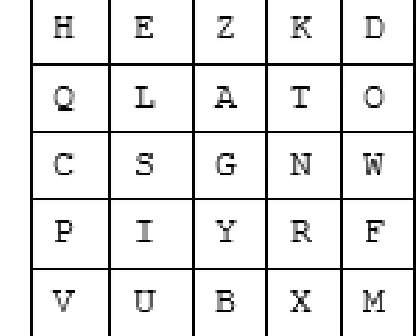
\includegraphics[width=0.4\linewidth, height=0.4\textheight, keepaspectratio]{figures/playfair-matriks.png}
    \caption{Matriks kunci Playfair berukuran $5 \times 5$; salah satu huruf --- biasanya \code{J} --- tidak dimuat sehingga matriks dapat menampung 26 huruf alfabet}
    \label{fig:playfair-matriks}
    \sumber{Munir, \textit{IF4020 Kriptografi}, ITB.}
\end{figure}

\textbf{Pemrosesan awal plainteks.} Sebelum dienkripsi, plainteks diolah
melalui lima langkah berikut.
\begin{enumerate}
    \item Buang seluruh spasi dan tanda baca.
    \item Ganti setiap huruf \code{J} menjadi \code{I}.
    \item Tuliskan hasilnya sebagai rangkaian bigram (pasangan dua huruf).
    \item Jangan biarkan sebuah bigram memuat dua huruf yang sama; bila terjadi,
          sisipkan huruf \code{X} di antara keduanya.
    \item Bila panjangnya ganjil setelah langkah-langkah di atas, tambahkan
          huruf \code{X} pada bigram terakhir.
\end{enumerate}
Langkah 4 dan 5 diperlukan karena aturan enkripsi Playfair tidak
mendefinisikan apa yang harus dilakukan bila kedua huruf bigram berada pada
sel yang sama.

\textbf{Aturan enkripsi.} Untuk setiap bigram, aturan yang berlaku bergantung
pada posisi kedua hurufnya di dalam matriks, sebagaimana dirangkum pada
Tabel~\ref{tab:playfair-aturan}.

\begin{table}[htbp]
\centering
\small
\begin{tabularx}{\linewidth}{@{}>{\raggedright\arraybackslash}p{3.4cm} >{\raggedright\arraybackslash}X >{\raggedright\arraybackslash}p{2.6cm}@{}}
\hline
\textbf{Posisi kedua huruf} & \textbf{Aturan} & \textbf{Contoh} \\
\hline
Baris yang sama & Ganti setiap huruf dengan huruf di kanannya, siklik kembali
ke awal baris & \code{di} $\rightarrow$ \code{FK}; \code{qt} $\rightarrow$
\code{RM} \\[4pt]
Kolom yang sama & Ganti setiap huruf dengan huruf di bawahnya, siklik kembali
ke awal kolom & \code{nq} $\rightarrow$ \code{PX}; \code{ow} $\rightarrow$
\code{WL} \\[4pt]
Membentuk persegi panjang & Huruf pertama menjadi huruf pada barisnya sendiri
dan kolom huruf kedua; huruf kedua menjadi huruf pada baris huruf kedua dan
kolom huruf pertama & \code{hz} $\rightarrow$ \code{BW}; \code{IH}
$\rightarrow$ \code{MB} \\
\hline
\end{tabularx}
\caption{Tiga aturan enkripsi Playfair cipher beserta contohnya}
\label{tab:playfair-aturan}
\sumber{Data dari Munir, \textit{IF4020 Kriptografi}, ITB.}
\end{table}

\textbf{Contoh terhitung.} Misalkan plainteksnya adalah \code{temui ibu nanti
malam}. Setelah spasi dibuang tersisa 18 huruf, dan setelah diperiksa ternyata
tidak ada huruf \code{J}, sehingga tidak ada penggantian yang diperlukan.
Perhatikan bahwa huruf ke-5 dan ke-6 berturut-turut adalah \code{i} dan
\code{i}, yang akan membentuk bigram kembar; karena itu disisipkan huruf
\code{X} di antaranya. Bigram yang dihasilkan adalah
\begin{center}
\texttt{te mu ix ib un an ti ma la mx},
\end{center}
dengan huruf \code{X} pada bigram terakhir ditambahkan karena jumlah hurufnya
semula ganjil. Penerapan aturan pada matriks kunci di atas menghasilkan
cipherteks
\begin{center}
\texttt{ZB RS FY KU PG LG RK VS NL QV}.
\end{center}
Sebagai pemeriksaan, ambil bigram pertama \code{te}: huruf \code{t} berada pada
baris 4 kolom 5, sedangkan \code{e} berada pada baris 1 kolom 5. Keduanya
berada pada kolom yang sama (\code{E}, \code{B}, \code{K}, \code{T},
\code{Z}), sehingga masing-masing diganti oleh huruf di bawahnya: \code{t}
menjadi \code{Z} dan \code{e} menjadi \code{B}, sesuai dengan cipherteks
\code{ZB}. Aturan persegi panjang diperlihatkan pada
Gambar~\ref{fig:playfair-baris}, sedangkan contoh enkripsi bigram \code{te}
diperlihatkan pada Gambar~\ref{fig:playfair-contoh}.

\begin{figure}[htbp]
    \centering
    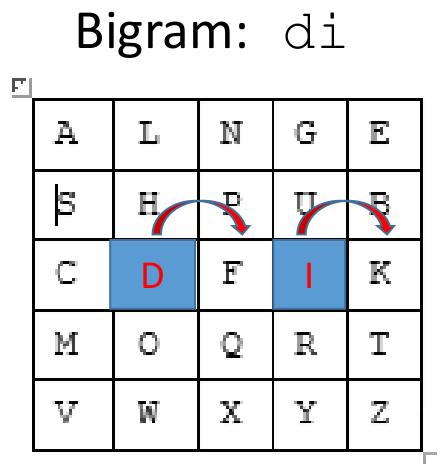
\includegraphics[width=0.32\linewidth, height=0.4\textheight, keepaspectratio]{figures/playfair-baris.png}
    \caption{Penerapan aturan baris yang sama pada Playfair cipher: huruf diganti oleh huruf di kanannya, dan siklik kembali ke awal baris bila sudah di ujung}
    \label{fig:playfair-baris}
    \sumber{Munir, \textit{IF4020 Kriptografi}, ITB.}
\end{figure}

\begin{figure}[htbp]
    \centering
    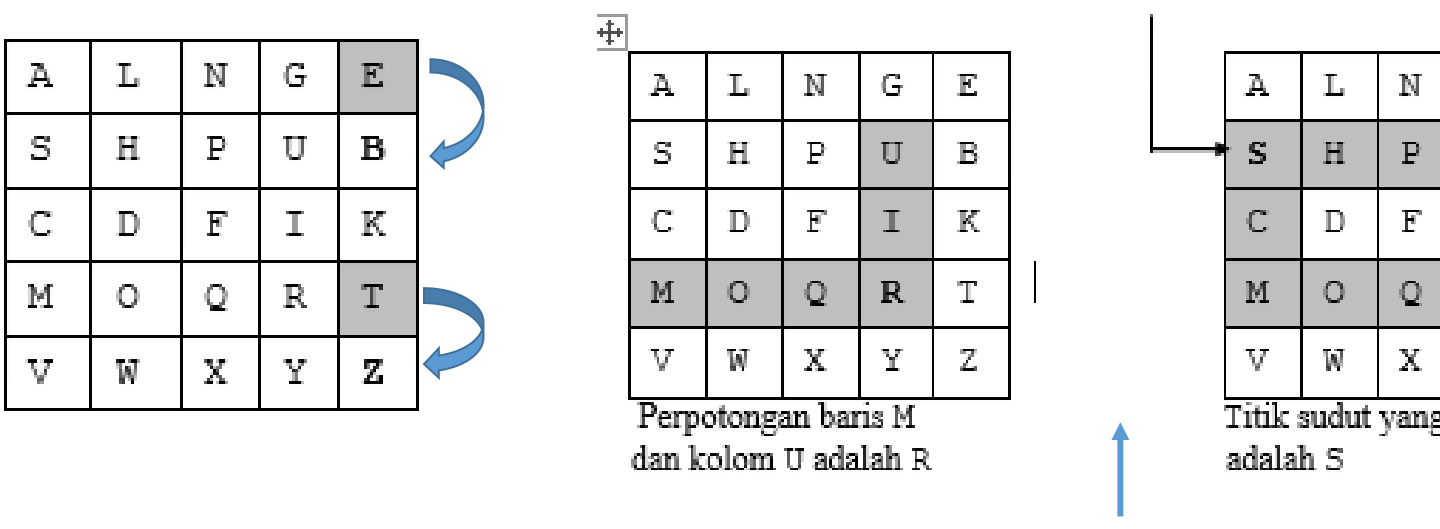
\includegraphics[width=0.9\linewidth, height=0.35\textheight, keepaspectratio]{figures/playfair-contoh.png}
    \caption{Enkripsi bigram \code{te} pada matriks kunci Playfair: karena kedua huruf berada pada satu kolom, masing-masing diganti huruf di bawahnya sehingga menjadi \code{ZB}}
    \label{fig:playfair-contoh}
    \sumber{Munir, \textit{IF4020 Kriptografi}, ITB.}
\end{figure}

\textbf{Dekripsi.} Dekripsi adalah kebalikan dari enkripsi: untuk baris yang
sama, huruf diganti dengan huruf di kirinya; untuk kolom yang sama, huruf
diganti dengan huruf di atasnya; sedangkan aturan persegi panjang berlaku
sama seperti pada enkripsi. Setelah dekripsi, huruf \code{X} pengisi yang
tidak bermakna dibuang, dan spasi ditambahkan kembali berdasarkan konteks
pesan.

\textbf{Kriptanalisis Playfair.} Dengan 26 huruf, jumlah bigram yang mungkin
adalah $26 \times 26 = 676$; setiap huruf plainteks kini selalu menjadi bagian
dari sebuah bigram, sehingga identifikasi huruf tunggal menjadi jauh lebih
sulit. Namun Playfair tetap dapat dipecahkan dengan \emph{analisis frekuensi
bigram}, karena sebaran bigram bahasa tetap lolos ke dalam cipherteks.
Bigram \code{TH} dan \code{HE} adalah bigram yang tersering di dalam bahasa
Inggris, sehingga keduanya menjadi tebakan pertama. Kelemahan tambahan yang
khas Playfair adalah \emph{aturan persegi panjang bersifat simetris terhadap
pembalikan}: bigram \code{AB} dan \code{BA} menghasilkan pola terenkripsi yang
saling membalik pula. Akibatnya pola bigram terbalik di dalam bahasa Inggris
--- misalnya \code{RE} dan \code{ER} seperti pada kata \emph{receiveR} dan
\emph{departED} --- tetap muncul dan dapat dikenali
\citep{stinson2018}. Sebagai gambaran langkahnya: bila \code{BM} adalah bigram
cipherteks yang paling sering, sedangkan \code{TH} adalah bigram plainteks
yang paling sering, penyerang berhipotesis bahwa \code{TH} dipetakan ke
\code{BM}. Bila enkripsi terjadi melalui aturan persegi panjang, maka huruf
\code{T} dan \code{B} berada pada satu baris, sedangkan \code{H} dan \code{M}
berada pada baris lain, dan dari situ sebagian matriks dapat direkonstruksi.
Setiap tebakan baru mempersempit kemungkinan matriks sampai seluruhnya
terbuka.

\subsection{Hill Cipher}
\label{sec:hill}

Hill cipher adalah polygram cipher berbasis aljabar linier. Cipher ini
dikembangkan oleh Lester S. Hill pada 1929 dan merupakan cipher klasik
pertama yang menggunakan operasi matriks secara sistematis
\citep{stinson2018}. Pada Hill cipher, $m$ huruf plainteks sekaligus diubah
menjadi $m$ huruf cipherteks melalui $m$ persamaan linier yang saling
bergantung.

Untuk $m = 3$, misalnya, sistem persamaannya adalah
\[
\begin{aligned}
c_1 &= (k_{11} p_1 + k_{12} p_2 + k_{13} p_3) \bmod 26,\\
c_2 &= (k_{21} p_1 + k_{22} p_2 + k_{23} p_3) \bmod 26,\\
c_3 &= (k_{31} p_1 + k_{32} p_2 + k_{33} p_3) \bmod 26,
\end{aligned}
\]
yang dapat dituliskan secara ringkas sebagai perkalian matriks
\begin{equation}
    \mathbf{C} = \mathbf{KP} \pmod{26},
    \label{eq:hill}
\end{equation}
dengan $\mathbf{K}$ adalah matriks kunci berukuran $m \times m$ dan
$\mathbf{P}$ adalah vektor kolom yang menyatakan blok plainteks. Gambaran
matriks untuk $m = 3$ diperlihatkan pada Gambar~\ref{fig:hill-matriks}.
Dekripsi membutuhkan invers matriks kunci $\mathbf{K}^{-1} \pmod{26}$, yang
hanya ada jika $\det(\mathbf{K})$ relatif prima dengan 26. Inilah alasan
mengapa tidak setiap matriks dapat dipakai sebagai kunci: bila
$\gcd(\det(\mathbf{K}), 26) \ne 1$, invers modulo 26 tidak ada dan cipherteks
tidak dapat dikembalikan.

\begin{figure}[htbp]
    \centering
    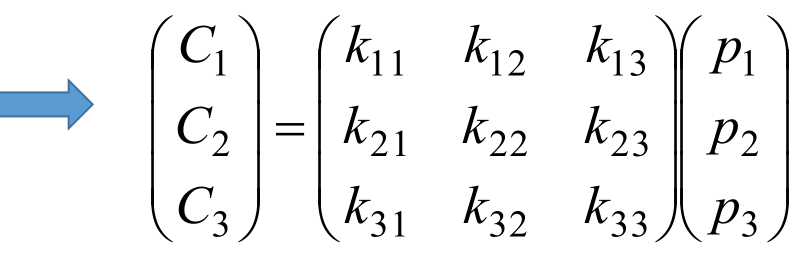
\includegraphics[width=0.7\linewidth, height=0.3\textheight, keepaspectratio]{figures/hill-matriks.png}
    \caption{Representasi matriks dari sistem persamaan linier Hill cipher untuk $m=3$; cipherteks diperoleh sebagai $\mathbf{C}=\mathbf{KP} \bmod 26$}
    \label{fig:hill-matriks}
    \sumber{Munir, \textit{IF4020 Kriptografi}, ITB.}
\end{figure}

\textbf{Contoh terhitung $m=3$.} Misalkan matriks kuncinya adalah
\[
\mathbf{K} =
\begin{pmatrix}
17 & 17 & 5\\
21 & 18 & 21\\
2  & 2  & 19
\end{pmatrix}
\]
dan plainteksnya \code{paymoremoney}. Kelompok pertama adalah \code{pay},
yaitu $\mathbf{P} = (15, 0, 24)^T$. Perkalian matriks menghasilkan
\[
\mathbf{KP} =
\begin{pmatrix}
17 \cdot 15 + 17 \cdot 0 + 5 \cdot 24\\
21 \cdot 15 + 18 \cdot 0 + 21 \cdot 24\\
2 \cdot 15 + 2 \cdot 0 + 19 \cdot 24
\end{pmatrix}
=
\begin{pmatrix}
375\\ 819\\ 486
\end{pmatrix}
\bmod 26
=
\begin{pmatrix}
11\\ 13\\ 18
\end{pmatrix}
=
\text{\code{LNS}}.
\]
Meneruskan cara yang sama untuk seluruh blok menghasilkan cipherteks
\begin{center}
\texttt{LNSHDLEWMTRW}.
\end{center}

Dekripsi memakai $\mathbf{K}^{-1}$, yang memenuhi
$\mathbf{K}\mathbf{K}^{-1} = \mathbf{I}$. Untuk matriks di atas,
\[
\mathbf{K}^{-1} =
\begin{pmatrix}
4  & 9  & 15\\
15 & 17 & 6\\
24 & 0  & 17
\end{pmatrix}.
\]
Sebagai pemeriksaan, dekripsi cipherteks \code{LNS} $= (11,13,18)^T$:
\[
\begin{pmatrix}
4 & 9 & 15\\
15 & 17 & 6\\
24 & 0 & 17
\end{pmatrix}
\begin{pmatrix}11\\13\\18\end{pmatrix}
=
\begin{pmatrix}431\\494\\570\end{pmatrix}
\bmod 26
=
\begin{pmatrix}15\\0\\24\end{pmatrix}
=
\text{\code{PAY}},
\]
kembali ke plainteks semula. Uji lain adalah memeriksa bahwa
$\mathbf{K}\mathbf{K}^{-1} \bmod 26$ benar-benar matriks identitas; perkalian
baris pertama dengan kolom pertama memberi
$17\cdot4 + 17\cdot15 + 5\cdot24 = 443 \equiv 1 \pmod{26}$, seperti
diperlihatkan pada Gambar~\ref{fig:hill-invers-3x3}.

\begin{figure}[htbp]
    \centering
    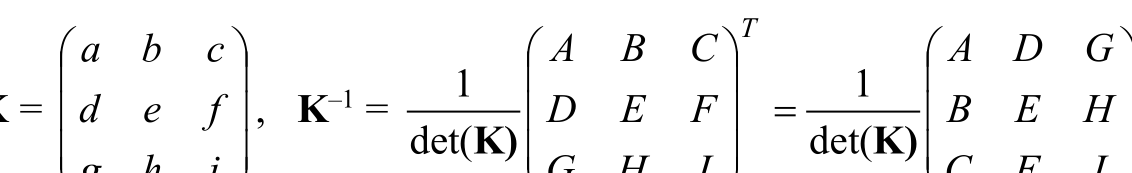
\includegraphics[width=0.95\linewidth, height=0.2\textheight, keepaspectratio]{figures/hill-invers-3x3.png}
    \caption{Rumus umum invers matriks $3\times3$ melalui determinan dan matriks kofaktor yang ditranspose; rumus inilah yang dipakai menghitung $\mathbf{K}^{-1}$ pada Hill cipher}
    \label{fig:hill-invers-3x3}
    \sumber{Munir, \textit{IF4020 Kriptografi}, ITB.}
\end{figure}

\textbf{Rumus invers untuk $m=2$.} Untuk matriks $2 \times 2$
$\mathbf{K} = \begin{pmatrix} a & b\\ c & d\end{pmatrix}$ dengan
$\det(\mathbf{K}) = ad - bc$, invers modulo 26 dihitung sebagai
\[
\mathbf{K}^{-1} = \frac{1}{\det(\mathbf{K})}
\begin{pmatrix} d & -b\\ -c & a\end{pmatrix}
= \bigl(\det(\mathbf{K})\bigr)^{-1}
\begin{pmatrix} d & -b\\ -c & a\end{pmatrix}.
\]
Sebagai contoh, ambil
$\mathbf{K} = \begin{pmatrix} 3 & 10\\ 15 & 9\end{pmatrix}$. Determinannya
adalah $\det(\mathbf{K}) = 3 \cdot 9 - 15 \cdot 10 = 27 - 150 = -123 \equiv 7
\pmod{26}$. Karena $7 \cdot 15 = 105 \equiv 1 \pmod{26}$, maka
$7^{-1} \equiv 15 \pmod{26}$. Dengan $-10 \equiv 16$ dan $-15 \equiv 11$,
diperoleh
\[
\mathbf{K}^{-1} = 15 \begin{pmatrix} 9 & 16\\ 11 & 3\end{pmatrix}
= \begin{pmatrix} 135 & 240\\ 165 & 45\end{pmatrix} \bmod 26
= \begin{pmatrix} 5 & 6\\ 9 & 19\end{pmatrix}.
\]
Uji balik: $\mathbf{K}\mathbf{K}^{-1} = \begin{pmatrix} 105 & 208\\ 156 &
261\end{pmatrix} \bmod 26 = \begin{pmatrix} 1 & 0\\ 0 & 1\end{pmatrix}$, yaitu
matriks identitas sebagaimana diharapkan.

Untuk $m = 3$, invers dihitung melalui matriks kofaktor. Bila
\[
\mathbf{K} = \begin{pmatrix} a & b & c\\ d & e & f\\ g & h & i\end{pmatrix},
\]
maka
\[
\mathbf{K}^{-1} = \frac{1}{\det(\mathbf{K})}
\begin{pmatrix}
A & B & C\\ D & E & F\\ G & H & I
\end{pmatrix},
\]
dengan kofaktor-kofaktornya adalah
\[
\begin{aligned}
A &= ei - hf, & B &= -(di - fg), & C &= dh - eg,\\
D &= -(bi - hc), & E &= ai - cg, & F &= -(ah - bg),\\
G &= bf - ec, & H &= -(af - cd), & I &= ae - bd,
\end{aligned}
\]
dan $\det(\mathbf{K}) = aA + bB + cC$. Karena seluruh operasi berlangsung
dalam modulo 26, hasil akhir setiap kofaktor harus direduksi kembali ke
rentang $0$ sampai $25$ \citep{stinson2018}.

\textbf{Kriptanalisis Hill cipher (serangan plaintext diketahui).} Hill
cipher berhasil menyembunyikan frekuensi huruf tunggal dengan sangat baik:
huruf plainteks yang sama pada posisi berbeda di dalam blok menghasilkan
huruf cipherteks yang berbeda. Namun sifat itu tidak cukup, karena Hill cipher
bersifat \emph{linier}. Bila penyerang mengetahui beberapa pasangan plainteks
dan cipherteks, ia dapat menuliskan hubungan
\[
\mathbf{K} = \mathbf{C}\,\mathbf{P}^{-1} \pmod{26}
\]
dan menghitung kuncinya secara langsung, tanpa pencarian sama sekali.

Sebagai contoh, misalkan untuk $m = 2$ penyerang mengetahui dua pasangan:
plainteks $P = (19,7)$ menghasilkan cipherteks $C = (0,23)$, dan plainteks
$P = (4,17)$ menghasilkan cipherteks $C = (12,6)$. Susun kedua vektor menjadi
kolom-kolom matriks:
\[
\mathbf{P} = \begin{pmatrix} 19 & 4\\ 7 & 17\end{pmatrix},
\qquad
\mathbf{C} = \begin{pmatrix} 0 & 12\\ 23 & 6\end{pmatrix}.
\]
Determinan $\mathbf{P}$ adalah $19\cdot17 - 4\cdot7 = 295 \equiv 9
\pmod{26}$, dan karena $9^{-1} \equiv 3 \pmod{26}$, inversnya adalah
\[
\mathbf{P}^{-1} = 3\begin{pmatrix} 17 & -4\\ -7 & 19\end{pmatrix}
= \begin{pmatrix} 51 & 66\\ 57 & 57\end{pmatrix} \bmod 26
= \begin{pmatrix} 25 & 14\\ 5 & 5\end{pmatrix}.
\]
Kuncinya kemudian diperoleh sebagai
\[
\mathbf{K} = \mathbf{C}\mathbf{P}^{-1}
= \begin{pmatrix} 0 & 12\\ 23 & 6\end{pmatrix}
\begin{pmatrix} 25 & 14\\ 5 & 5\end{pmatrix}
=
\begin{pmatrix} 60 & 60\\ 605 & 352\end{pmatrix} \bmod 26
=
\begin{pmatrix} 8 & 8\\ 7 & 14\end{pmatrix}.
\]
Langkah-langkah serangan ini diperlihatkan pada
Gambar~\ref{fig:hill-known-plaintext}. Uji balik dengan
$\mathbf{K} = \begin{pmatrix} 8 & 8\\ 7 & 14\end{pmatrix}$: untuk
$(19,7)$ diperoleh
$(8 \cdot 19 + 8 \cdot 7,\; 7 \cdot 19 + 14 \cdot 7) = (208, 231) \bmod 26 =
(0, 23)$, sesuai dengan cipherteks yang diketahui.

Pelajaran dari Hill cipher penting untuk bab-bab berikutnya. Kekuatan
kriptografis tidak lahir dari kerumitan operasi, melainkan dari ketiadaan
struktur yang dapat dieksploitasi. Cipher linier mudah dipecahkan justru
karena kelinierannya, dan prinsip inilah yang kemudian mendorong perancangan
cipher modern berbasis S-box yang tidak linier \citep{stinson2018}.

\begin{figure}[htbp]
    \centering
    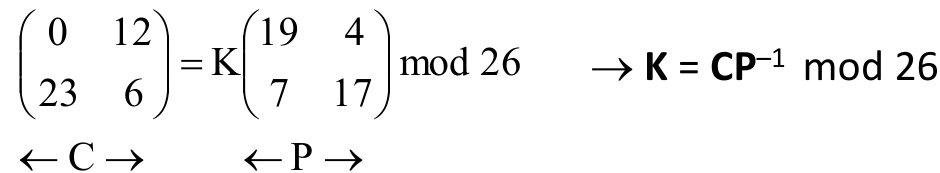
\includegraphics[width=0.9\linewidth, height=0.2\textheight, keepaspectratio]{figures/hill-known-plaintext.png}
    \caption{Kriptanalisis Hill cipher dengan serangan plaintext diketahui: kunci dihitung langsung sebagai $\mathbf{K}=\mathbf{C}\mathbf{P}^{-1} \bmod 26$}
    \label{fig:hill-known-plaintext}
    \sumber{Munir, \textit{IF4020 Kriptografi}, ITB.}
\end{figure}
